\chapter{Thu thập và Tiền xử lý dữ liệu}

\section{Phương án thu thập}

\subsection{Dữ liệu FireAnt}
Để thực hiện phân tích diễn đàn, ta cần cào dữ liệu là những bài đăng của người dùng lên diễn đàn đó.\\

FireAnt là diễn đàn đã tồn tại lâu đời, với hơn 3 triệu tài khoản đã được đăng ký \cite{fireant}. Do đó, chúng ta hoàn toàn có thể kì vọng một lượng bài đăng cũng như tương tác ổn định ở diễn đàn này.

\begin{figure}[h]
    \centering
    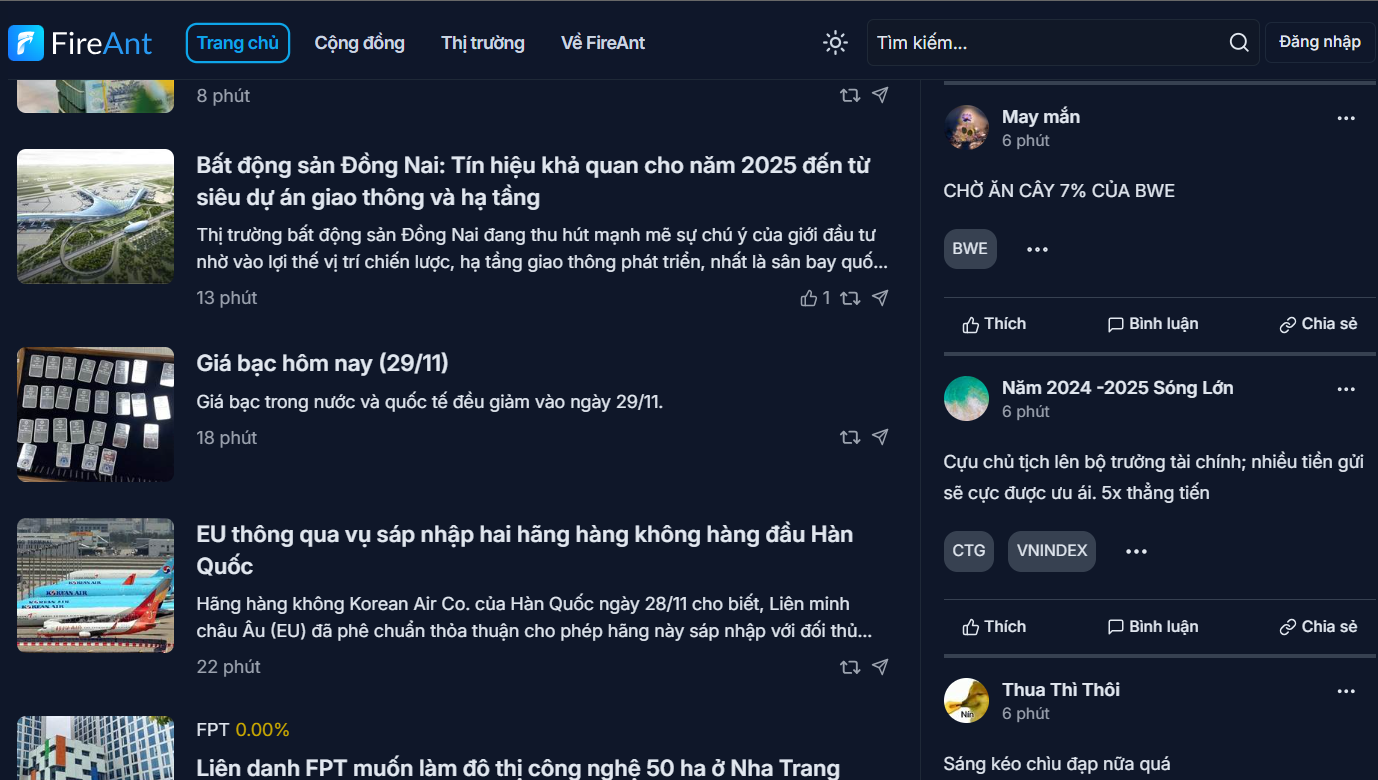
\includegraphics[width=0.9\textwidth]{images/fig-1.1-fireant.png}
    \caption{Trang chủ của FireAnt}
    \label{fig:1.1}
\end{figure}

Tất nhiên, do lượng dữ liệu từ toàn bộ các bài đăng của trang này là quá khổng lồ, chúng ta sẽ chỉ thu thập những bài đăng gần đây nhất. Ở đây ta hi vọng có thể thu được dữ liệu trong khoảng thời gian \textbf{hai tháng}, đặc biệt tại thời điểm thị trường có nhiều biến động.\\

Nền tảng FireAnt cung cấp cho người dùng một bộ API tương đối đầy đủ, có thể truy cập bằng cách gửi request vào đường dẫn \href{https://api.fireant.vn/}{https://api.fireant.vn/}.\\

API này yêu cầu một Authentication Token của người dùng, tuy nhiên ta có thể tạo một tài khoản và lấy Token của tài khoản đó một cách dễ dàng.\\

Như vậy, công việc thu thập dữ liệu từ FireAnt bao gồm các công đoạn sau:

\begin{enumerate}
    \item Cung cấp các thông tin cần thiết (Auth Token);
    \item Tiến hành gọi request, thu thập dữ liệu từ những thông tin được cung cấp;
    \item Xử lý dữ liệu, tái tổ chức và lưu trữ.
\end{enumerate}

\subsection{Dữ liệu Chứng khoán}
Tương tự, để khớp với dữ liệu trong FireAnt, ta cũng cần cào dữ liệu của thị trường trong khoảng thời gian đó. Ta hi vọng có thể thu được dữ liệu của toàn bộ các mã chứng khoán, các chỉ số nổi tiếng (VNINDEX, DJI, N225, ...), trong khoảng thời gian hai tháng, trùng với khoảng thời gian bên trên.\\

Một vài công ty chứng khoán như TCBS, Vietcap hay các trang tin như MSN Finance có sẵn bảng giá và lịch sử giá của các mã chứng khoán, và ta có thể lấy được chúng thông qua API và dữ liệu được cào trực tiếp trong trang.\\

Hơn nữa, xuất hiện một số thư viện có thể gọi API cũng như cào dữ liệu một cách tự động, tiêu biểu là thư viện \texttt{vnstocks} \cite{vnstocks}.\\

Như vậy, công việc thu thập dữ liệu chứng khoán bao gồm:

\begin{enumerate}
    \item Tải và cài đặt các thư viện cần thiết;
    \item Lên danh sách các mã cần quan tâm;
    \item Tiến hành chạy thư viện, thư viện sẽ gọi API và cào dữ liệu tương ứng;
    \item Xử lý dữ liệu, tái tổ chức và lưu trữ.
\end{enumerate}

\subsection{Công cụ}
Để hỗ trợ trong việc thu thập, xử lý dữ liệu, ta sử dụng những thư viện:

\begin{itemize}
    \item \texttt{vnstocks} cung cấp công cụ cần thiết để tự động cào, trích xuất dữ liệu từ các công ty chứng khoán;
    \item \texttt{requests, selenium} cung cấp khả năng gọi API, trích xuất dữ liệu từ trang web;
    \item \texttt{pandas, numpy, json, csv} cung cấp khả năng tổ chức, biến đổi dữ liệu, đọc dữ liệu JSON, đồng thời lưu trữ dữ liệu dưới dạng file CSV.
\end{itemize}

\section{Quá trình thu thập}
\subsection{Dữ liệu FireAnt}
Đầu tiên, ta tiến hành lấy Auth Token trong một request bằng chế độ Inspect trên trình duyệt.
\begin{center}
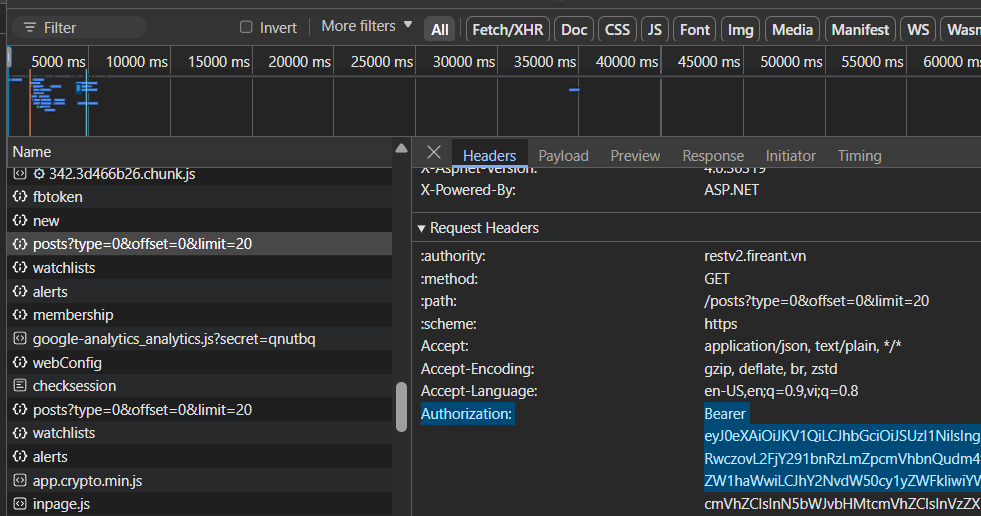
\includegraphics[width=0.9\textwidth]{images/code-1.1-inspect.png}
\end{center}

Dãy token này sẽ được sử dụng trong suốt quá trình thu thập.\\
\begin{center}
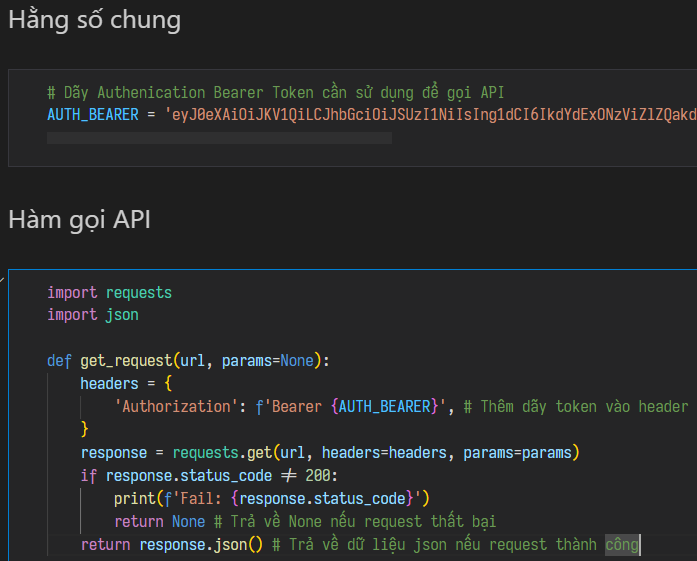
\includegraphics[width=0.6\textwidth]{images/code-1.2-getrequest.png}
\end{center}

Để thực hiện cào bài viết của người dùng, ta sẽ request tới \href{https://api.fireant.vn/posts}{https://api.fireant.vn/posts} cùng 3 tham số là \texttt{type}, \texttt{offset}, \texttt{limit}.

\begin{center}
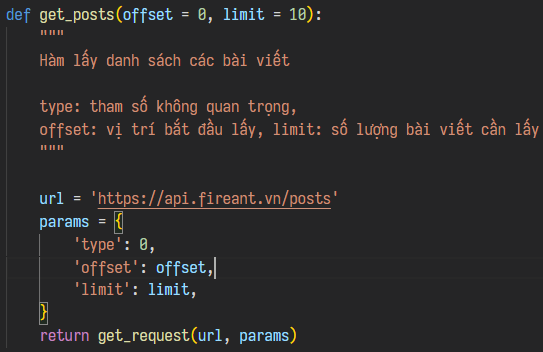
\includegraphics[width=0.6\textwidth]{images/code-1.3-getposts.png}
\end{center}

Để đảm bảo dữ liệu không xảy ra trùng lặp, sau mỗi lần gọi hàm, ta cần xét số bài viết đã lấy được và tính lại \texttt{offset}. Ngoài ra cần xét nếu dữ liệu nằm ngoài khoảng thời gian yêu cầu thì không lấy. Ta sẽ ghi lại dữ liệu này vào một file CSV.

\begin{center}
    \centering
    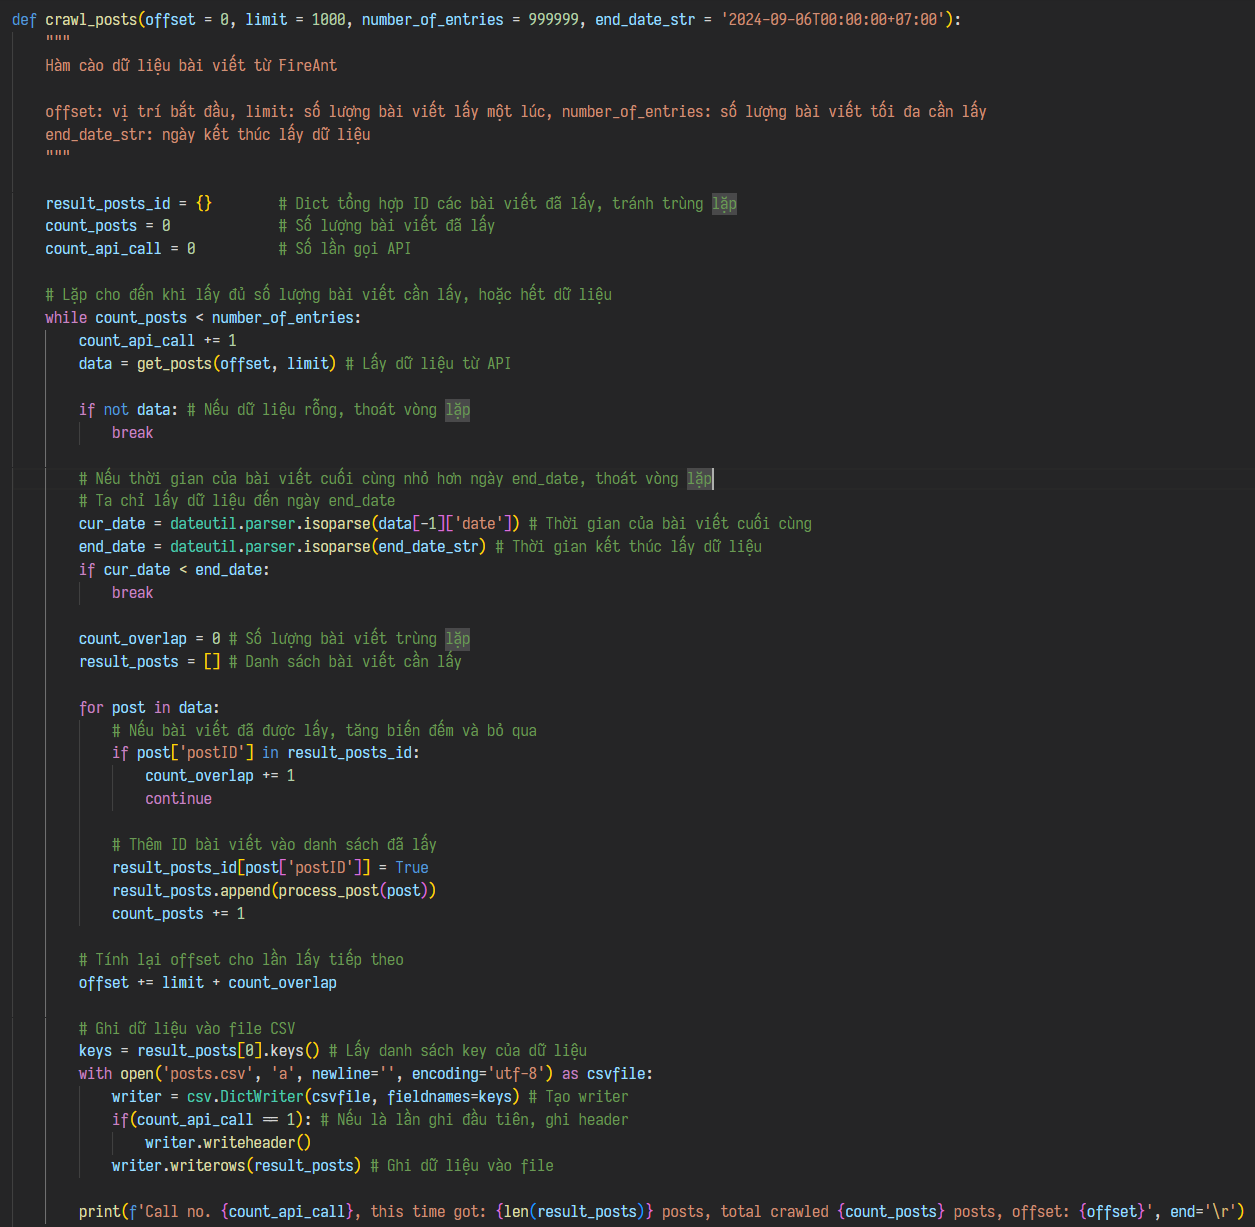
\includegraphics[width=1\linewidth]{images/code-1.4-crawlpost.png}
\end{center}

Ta thực hiện lấy \textbf{1000 bài viết} một lúc, lấy những bài viết kể từ \textbf{06/9/2024 cho tới 06/11/2024}. Tổng cộng cào được \textbf{272979 bài viết}.

\begin{center}
    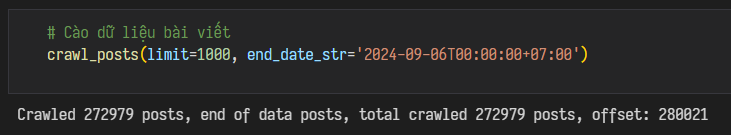
\includegraphics[width=1\linewidth]{images/code-1.6-crawlresult.png}
\end{center}

Dữ liệu trả về có dạng JSON, là một list gồm các phần tử là object đại diện cho bài viết, trong đó có 60 trường dữ liệu, nổi bật có ID bài viết, ngày đăng, thông tin người đăng, nội dung bài viết, tổng số lượt thích/chia sẻ/bình luận, mã chứng khoán được nhắc đến, tầm nhìn tích cực/tiêu cực (sentiment), link, hình ảnh, video (nếu có).\\

\begin{figure}[H]
  \begin{subfigure}{.4\textwidth}
  \centering
    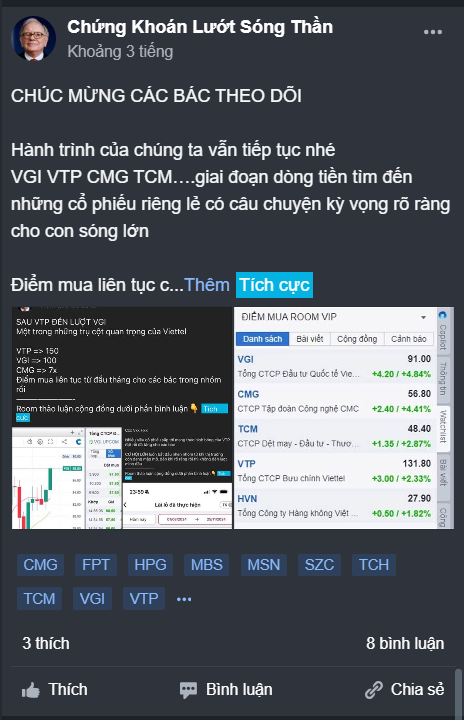
\includegraphics[width=1\linewidth]{images/fig-1.2.1-examplepost.png}
  \end{subfigure}%
  \begin{subfigure}{.55\textwidth}
  \centering
    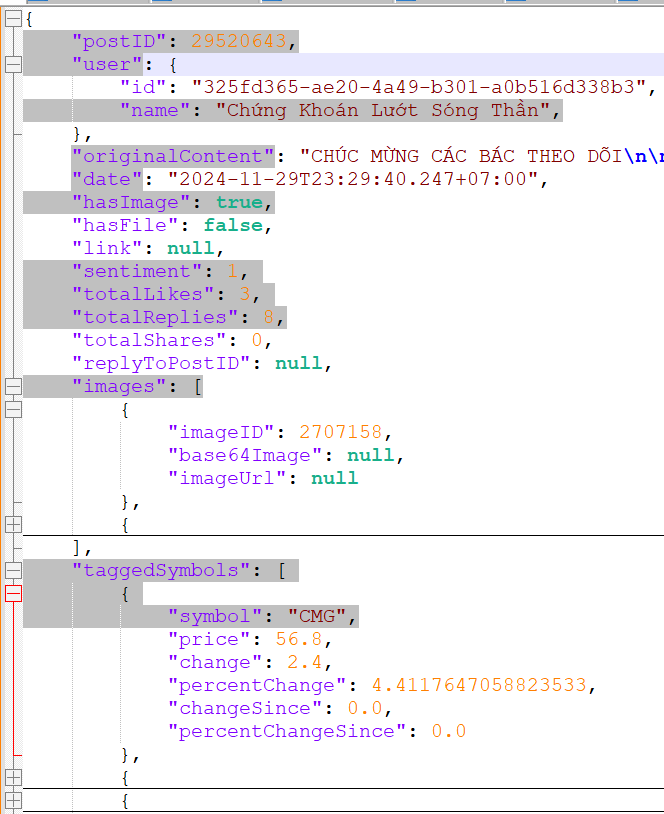
\includegraphics[width=1\linewidth]{images/fig-1.2.2-examplepostjson.png}
  \end{subfigure}
  \caption{Ví dụ một bài viết}
\end{figure}

Tuy nhiên, request trên không bao gồm dữ liệu về phần bình luận của bài viết. Với mỗi một bài viết, ta cần gửi một request để lấy bình luận của bài viết đó. Đường dẫn cần gửi tới là \href{https://api.fireant.vn/posts/\{post_id\}/replies}{https://api.fireant.vn/posts/<post-id>/replies}, với \texttt{<post-id>} là ID bài viết. Cấu trúc request tương tự như trên.

\begin{center}
    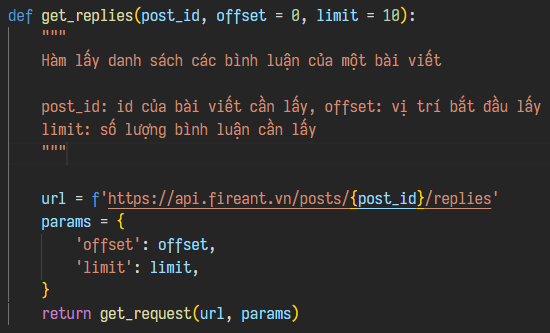
\includegraphics[width=0.6\linewidth]{images/code-1.7-crawlrep.png}
\end{center}

Ta cũng thực hiện gọi hàm này tương tự cách gọi hàm lấy bài viết. Do cấu trúc của bình luận và bài viết là như nhau (bình luận là một dạng bài viết), ta không cần xử lý thêm nhiều. Ta sẽ ghi lại dữ liệu này vào một file CSV khác.\\

Tuy nhiên, với số lượng bài viết lên tới 270 nghìn, việc gọi requests cho từng bài viết mất rất nhiều thời gian và có nguy cơ gây quá tải. Theo thống kê, \textbf{3418 bài viết có ít nhất 15 bình luận}. Vì vậy, ta chỉ cào dữ liệu bình luận trong những bài viết này. Ngoài ra, giữa các request sẽ có khoảng delay là 0.2 giây để tránh bị chặn IP.

\begin{center}
    \centering
    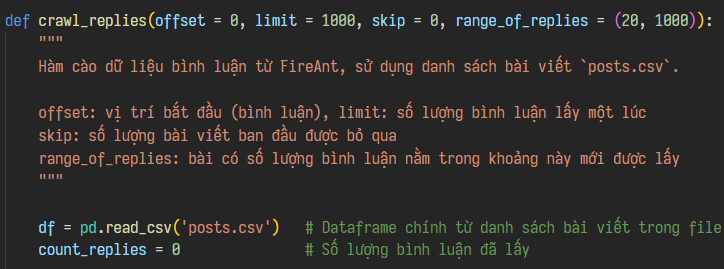
\includegraphics[width=0.7\linewidth]{images/code-1.8-crawlrep1.png}
    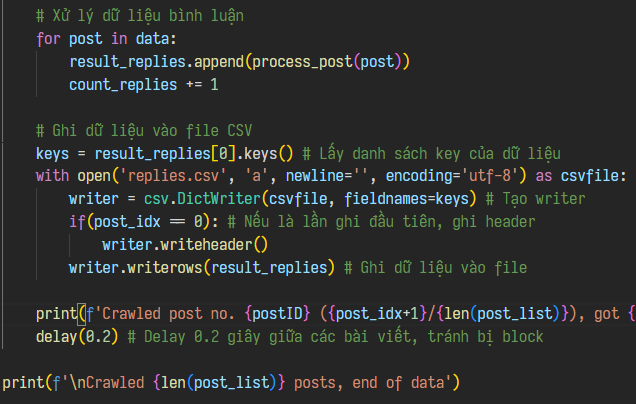
\includegraphics[width=0.7\linewidth]{images/code-1.9-crawlrep2.png}
\end{center}

Tổng cộng cào được \textbf{75510 bình luận} có trong \textbf{3418 bài viết}.
\begin{center}
    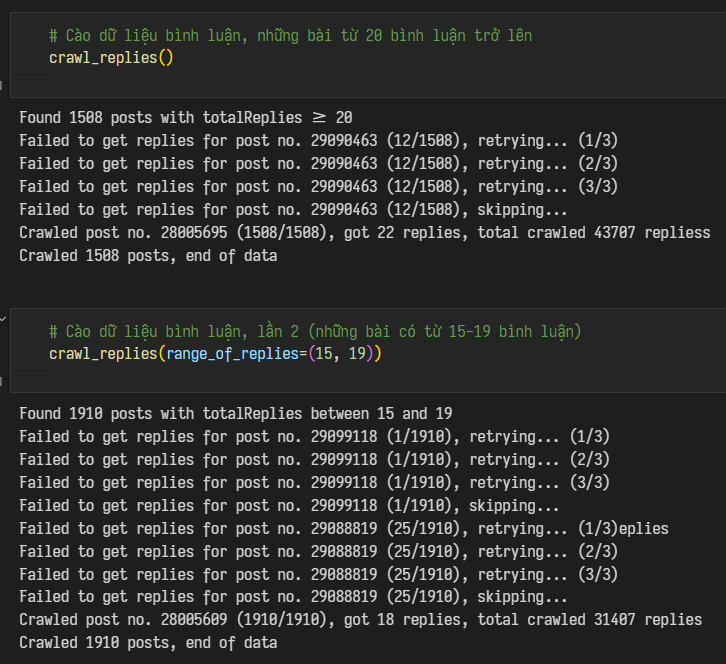
\includegraphics[width=0.8\linewidth]{images/code-1.10-crawlrepresult.png}
\end{center}

\subsection{Dữ liệu Chứng khoán}

Với việc có thư viện hỗ trợ, công việc cào dữ liệu chứng khoán tương đối đơn giản.

\begin{center}
    \centering
    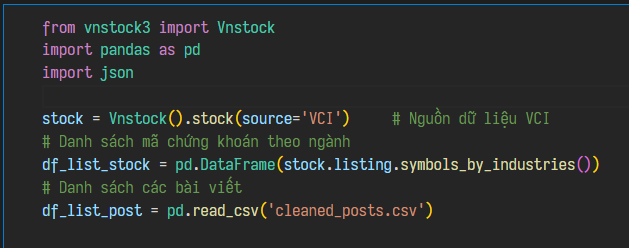
\includegraphics[width=0.75\linewidth]{images/code-1.11-crawllib.png}
\end{center}

\subsubsection*{Thông số cơ bản}
Với mỗi cổ phiếu, ta để tâm đến những dữ liệu đáng chú ý:
\begin{enumerate}
    \item Dữ liệu về tên công ty, ngành nghề:
    \begin{center}
        \centering
        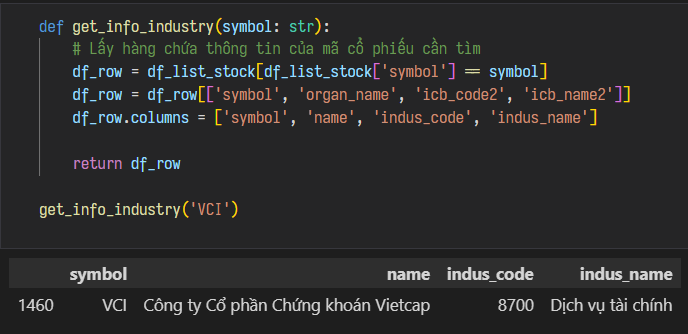
\includegraphics[width=0.75\linewidth]{images/code-1.12-crawlstock1.png}
    \end{center}
    \item Dữ liệu về số lượng cổ đông, nhân viên, đánh giá của TCBS:
    \begin{center}
        \centering
        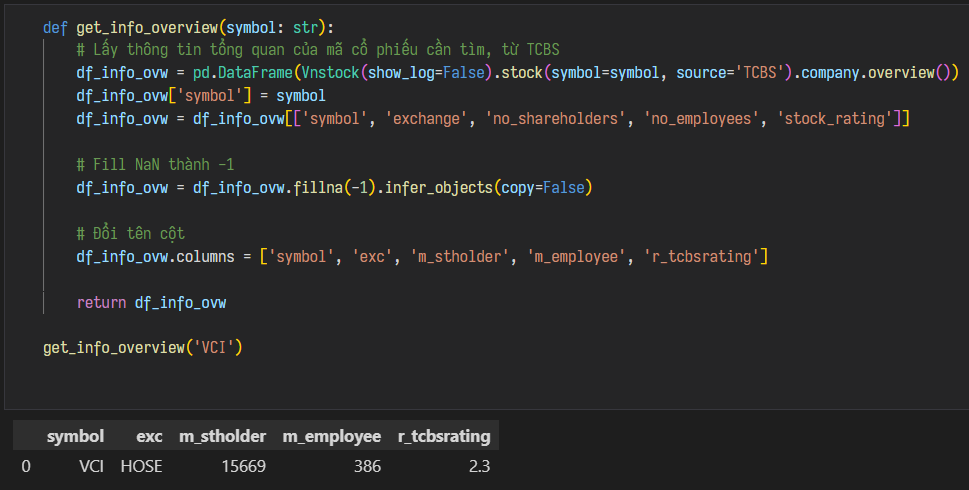
\includegraphics[width=1\linewidth]{images/code-1.13-crawlstock2.png}
    \end{center}
    \item Dữ liệu về thông tin tài chính công ty, các chỉ số tài chính:
    \begin{center}
        \centering
        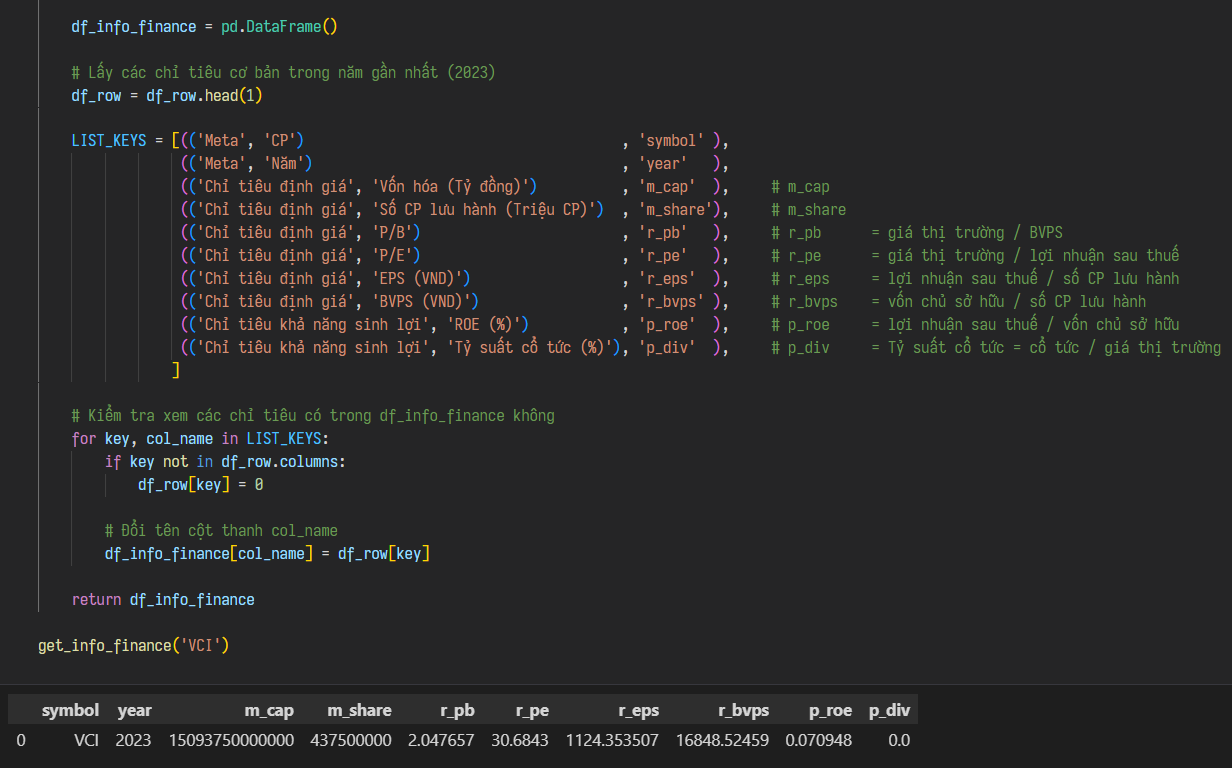
\includegraphics[width=1\linewidth]{images/code-1.14-crawlstock3.png}
    \end{center}
\end{enumerate}

Kết quả có \textbf{1528 mã cổ phiếu}, ta thực hiện lấy và gộp 3 miền dữ liệu bên trên:
\begin{center}
    \centering
    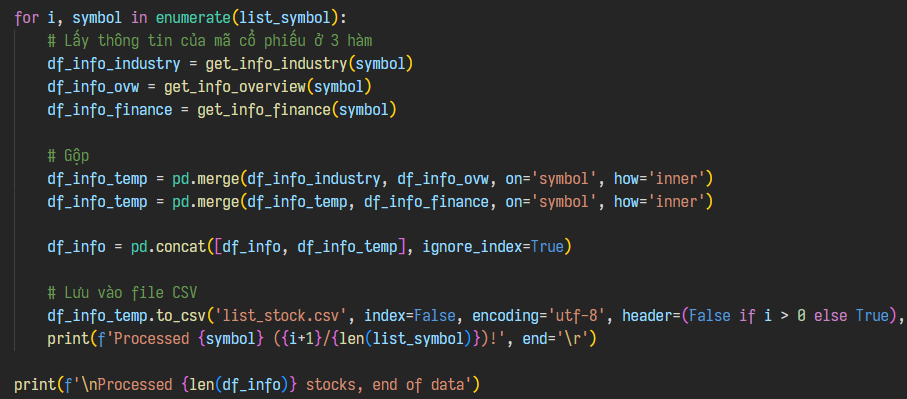
\includegraphics[width=0.8\linewidth]{images/code-1.15-crawlstockmerge.png}
    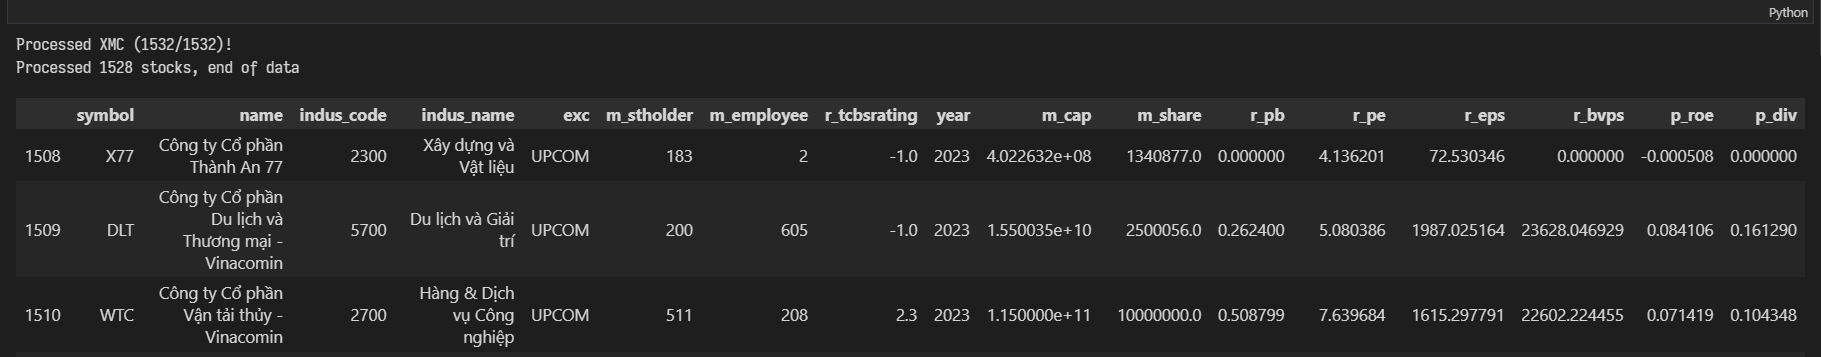
\includegraphics[width=1\linewidth]{images/code-1.16-crawlstockresult.png}
\end{center}

\subsubsection*{Lịch sử giá}
Ta lấy danh sách các mã cổ phiếu được đề cập trong danh sách bài viết. Ta chỉ thực hiện lấy lịch sử giá của các mã cổ phiếu, chỉ số nổi tiếng (VNINDEX, VN30, DJI, ...). Ta lấy dữ liệu từ ngày \textbf{01/9/2024} cho tới ngày \textbf{08/11/2024}.\\

Ta sẽ lấy lịch sử giá theo \textbf{khung thời gian 30 phút}. Mỗi mục trong lịch sử giá sẽ bao gồm giá khởi điểm (\texttt{open}), giá đóng khung (\texttt{close}), giá cao nhất trong khung (\texttt{high}), giá thấp nhất trong khung (\texttt{low}), khối lượng giao dịch (\texttt{volume}). Một số mã do không đủ dữ liệu, nên chỉ lấy trong khung thời gian 1 ngày.

\begin{center}
    \centering
    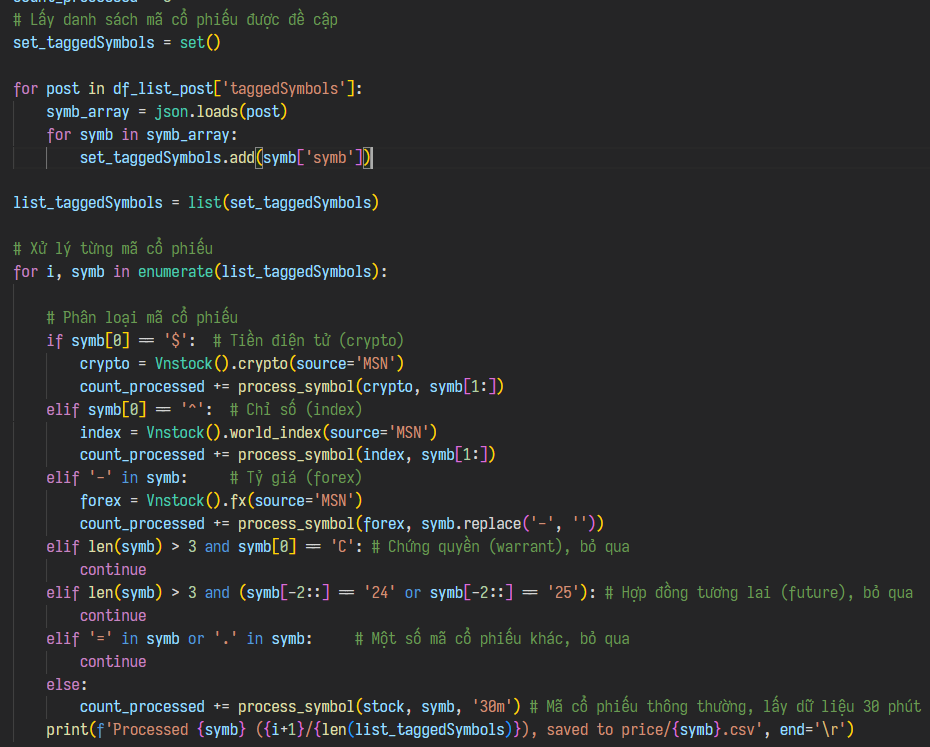
\includegraphics[width=1\linewidth]{images/code-1.17-crawlhistory.png}
\end{center}

Kết quả ta lấy được lịch sử giá của \textbf{1154 mã}, với mỗi mã đều có cấu trúc như trên:
\begin{center}
    \centering
    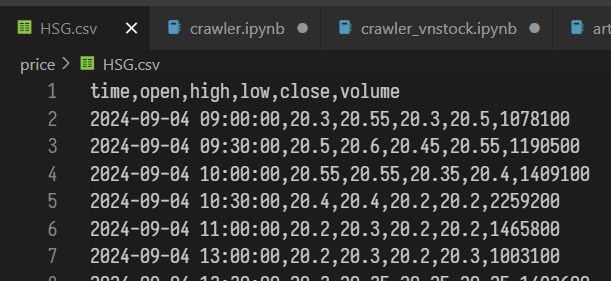
\includegraphics[width=0.6\linewidth]{images/code-1.18-crawlhistoryex.png}
\end{center}

\section{Tiền xử lý, làm sạch dữ liệu}
\subsubsection*{Dữ liệu FireAnt}
Trong 60 trường dữ liệu, ta chỉ phân tích một vài trường dữ liệu:
\begin{center}
    \centering
    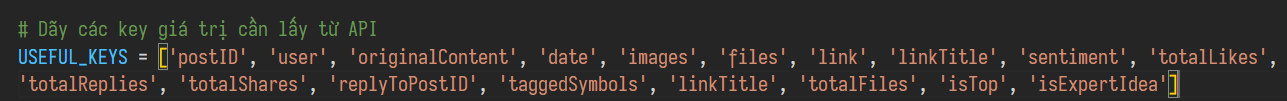
\includegraphics[width=1\linewidth]{images/code-1.19-filter.png}
\end{center}

Một vài trường dữ liệu chỉ có một giá trị, ví dụ như \texttt{totalShares} chỉ có giá trị 0 (?), \texttt{files, totalFiles} cũng không có giá trị, \texttt{isTop, isExpertIdea} toàn bộ là False...

\begin{center}
    \centering
    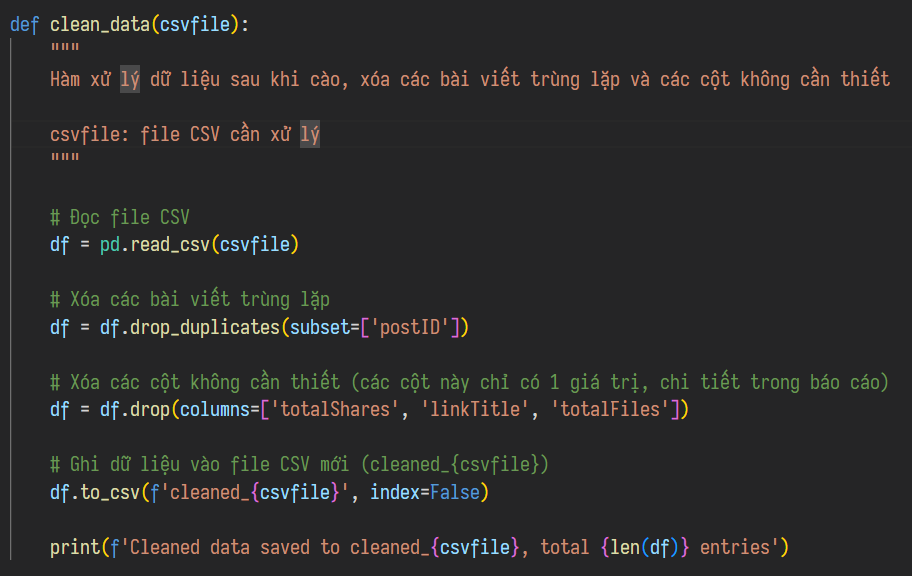
\includegraphics[width=0.8\linewidth]{images/code-1.20-filterstep2.png}
\end{center}

Một số trường dữ liệu có thể đơn giản hơn nữa, ví dụ như danh sách các mã chứng khoán được nhắc đến (\texttt{taggedSymbols}), thay vì lưu toàn bộ dữ liệu, ta thực sự chỉ quan tâm đến tên cổ phiếu và giá của cổ phiếu tại thời điểm dăng bài. Một số khác như \texttt{images, files}, ta chỉ cần quan tâm đến số lượng.

\begin{center}
    \centering
    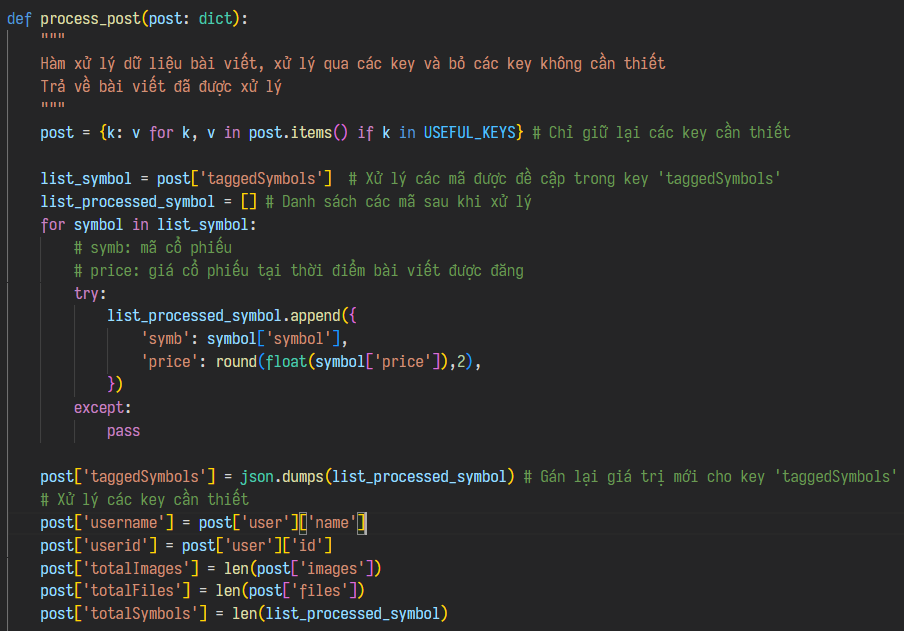
\includegraphics[width=0.85\linewidth]{images/code-1.21-filterstep3.png}
\end{center}

Bằng cách trên, kích cỡ dữ liệu đã giảm 4 lần, từ 417MB xuống còn 105MB.

\begin{center}
    \centering
    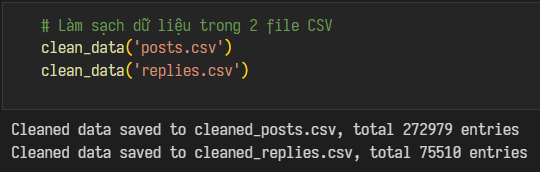
\includegraphics[width=0.7\linewidth]{images/code-1.22-filterresult.png}
\end{center}

Ngoài ra, một số bài viết bị nhảy, mất dữ liệu. Tuy nhiên có thể giải quyết bằng cách gửi request ID bài viết bị hụt đến API \href{https://api.fireant.vn/posts/<post-id>}{https://api.fireant.vn/posts/<post-id>}.\\

Với dữ liệu bình luận cũng xảy ra tình trạng tương tự. Nếu dữ liệu trả về Null, ta sẽ thử lại 3 lần, giữa mỗi lần delay sẽ tăng thêm. Nếu vẫn không lấy được dữ liệu, hoặc bị lỗi 403 Forbidden thì khả năng cao bị chặn IP, cần phải thử lại sau (và thực tế chúng em đã bị chặn IP hai lần).

\subsubsection*{Dữ liệu chứng khoán}
Dữ liệu thông số cơ bản của các công ty tương đối sạch.\\

Dữ liệu lịch sử giá tại các công ty chứng khoán Việt cũng rất ổn, tuy nhiên có một số mã phải cào ở nguồn MSN bị thiếu (các chỉ số quốc tế như DJI, giá tiền ảo như BTC...), chỉ có dữ liệu theo từng tháng.
\begin{center}
    \centering
    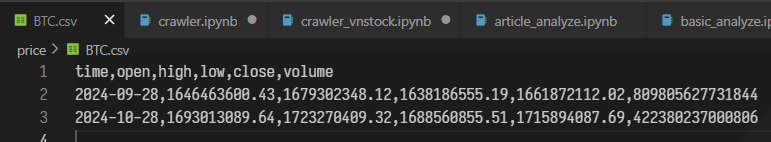
\includegraphics[width=0.75\linewidth]{images/code-1.23-abnormalex.png}
\end{center}

Ta cần tìm nguồn dữ liệu khác. Qua quá trình tìm hiểu, chúng em phát hiện trang \href{https://vn.investing.com}{https://vn.investing.com} có cung cấp giá lịch sử của loại mã này:

\begin{figure}[H]
    \centering
    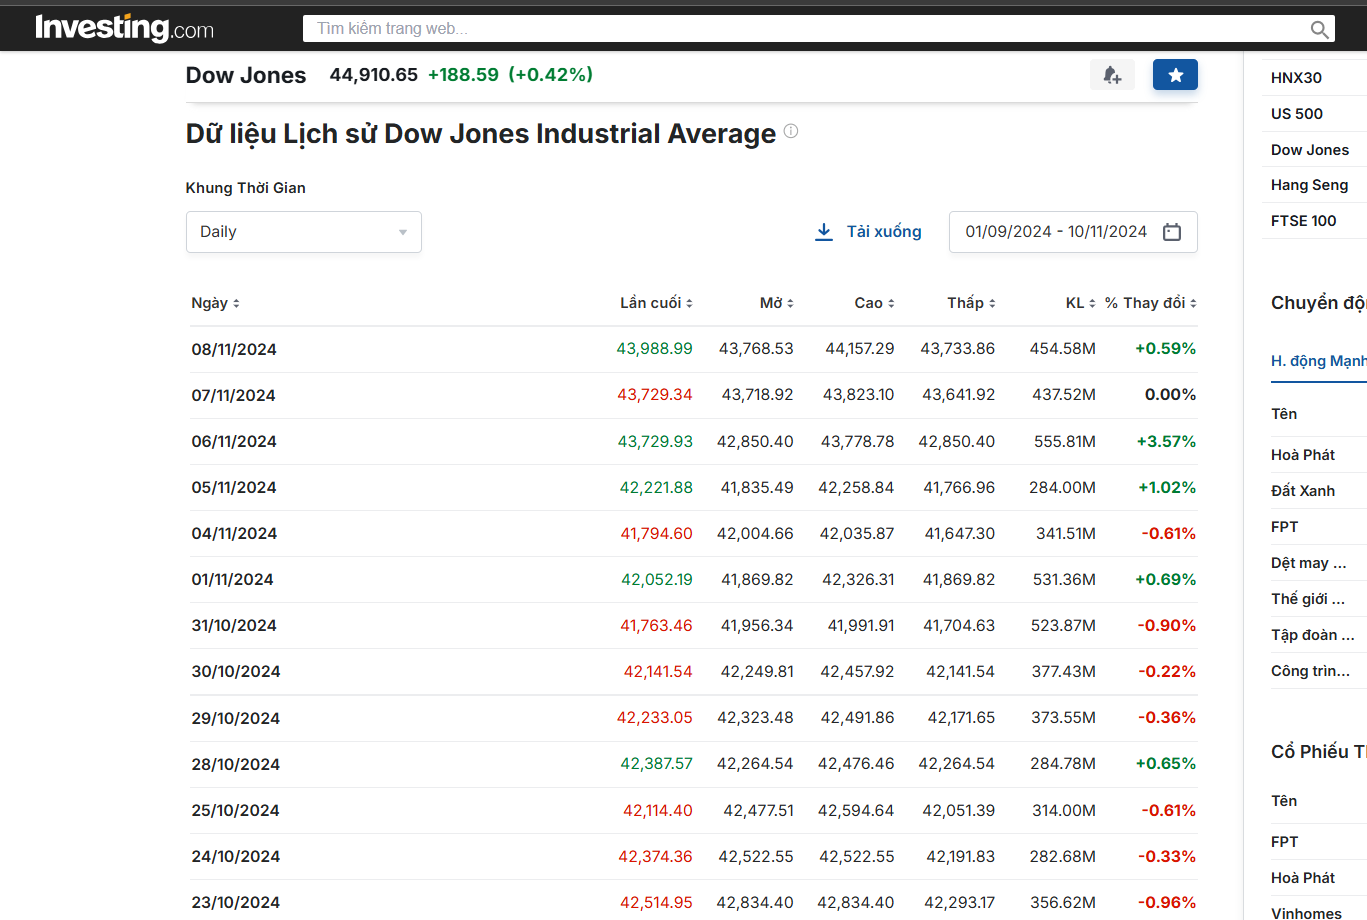
\includegraphics[width=1\linewidth]{images/fig-1.3-investinghomepage.png}
    \caption{Thông tin lịch sử giá trên trang Investing}
    \label{fig:1.3}
\end{figure}

Sử dụng công cụ Inspect, ta tìm ra được API để lấy giá lịch sử:
\begin{center}
    \centering
    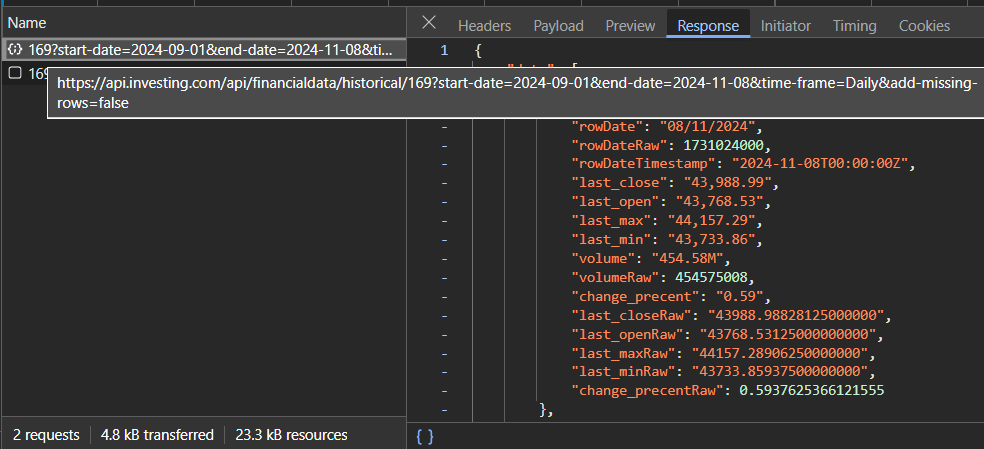
\includegraphics[width=0.9\linewidth]{images/code-1.24-inspectinv.png}
\end{center}

Ta tích hợp API này vào Notebook (\texttt{crawl\_indexes.ipynb}), xử lý kết quả để nó có dạng giống các mã khác, sau đó lưu vào một file CSV trong thư mục mới.
\begin{center}
    \centering
    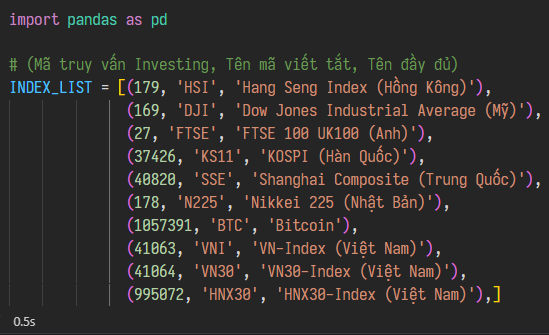
\includegraphics[width=0.6\linewidth]{images/code-1.25-crawlinvestingindex.png}
\end{center}


Tương tự, ta sẽ lấy dữ liệu từ ngày 01/9/2024 đến 08/11/2024.
\begin{center}
    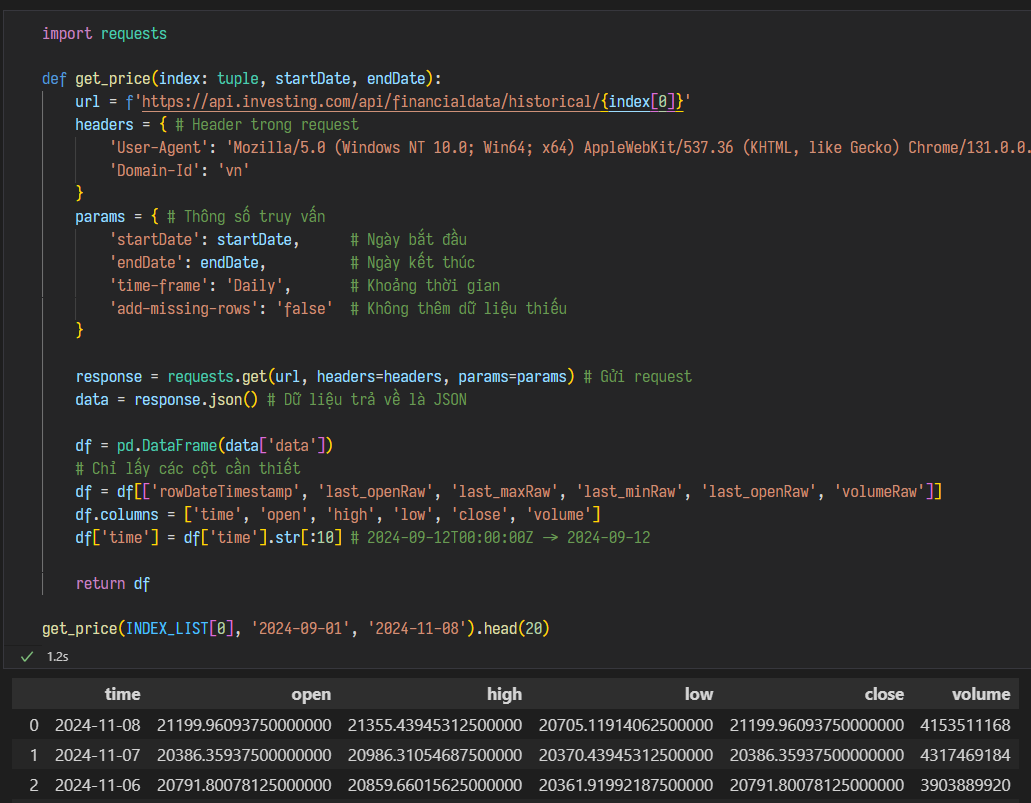
\includegraphics[width=0.75\linewidth]{images/code-1.26-crawlinvesting.png}
    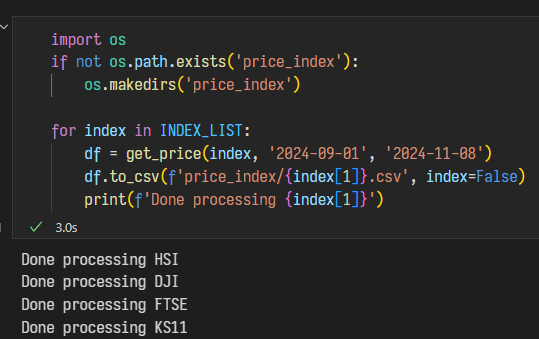
\includegraphics[width=0.6\linewidth]{images/code-1.27-crawlinvestingres.png}
    
\end{center}

Dữ liệu đã được bổ sung đầy đủ, ngoài ra còn có thêm dữ liệu của một số chỉ số không có trong dữ liệu ban đầu.
\begin{center}
    \centering
    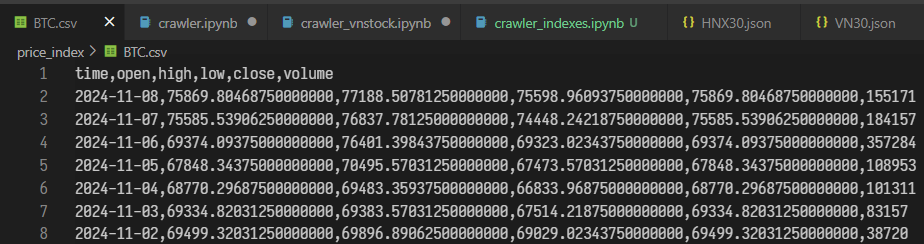
\includegraphics[width=1\linewidth]{images/code-1.28-crawlbtcresult.png}
\end{center}

\textbf{Ta kết thúc quá trình thu thập và tiền xử lý dữ liệu ở đây.} Tuy nhiên với một vài trường hợp cụ thể, ta vẫn cần phải xử lý thêm dữ liệu, để dữ liệu phù hợp với hướng phân tích đó.